\section{Eksperimentdesign}
Forskningsspørsmålet var følgende: \textit{Kan et system  basert på semantisk web-teknolgi hjelpe farmasøyter til å gjøre legemiddelgjennomgang slik at den blir mer presis, raskere gjennomført og lærerik?} For å kunne svare på forskningsspørsmålet planla vi å sammenligne presisjon, tidsbruk og læringseffekt av legemiddelgjennomganger med og uten forslag til tiltak. En prototype ble utviklet for dette formålet med navn \textit{SemLMG}. I dette delkapittelet vil plan for forskningsmetode, omgivelser og rekruttering av deltagere bli presentert. Videre vil eventuelle fordeler og ulemper ved disse valgene bli diskutert.  

\subsection{Valg av metode}
Valg av forskningsmetode måtte bero på muligheten til å sammenligne presisjon, tidsbruk og læringseffekt med og uten forslag til tiltak ved bruk av SemLMG. For å kunne sammenligne disse aspektene må de være målbare. Tidsbruk ville måles med å ta tiden brukt på gjennomføre legemiddelgjennomgangen. Definisjon på presisjon av legemiddelgjennomgang og læringseffekt ved bruk av prototypen vil bli diskutert her.

Måling av presisjon til en legemiddelgjennomgang har vært diskutert over lengre tid i denne masteroppgaven. Man har ingen klare mål på hva som gjør en legemiddelgjennomgang ''bedre''. Valg gjort i legemiddelgjennomganger er ikke kun avhengig av legemidler, men like mye pasientspesifikk informasjon som pasientens egne preferanser, allergier, hypersensitivitet og mer. Siden deltagerne skulle utføre legemiddelgjennomgang på de samme tilfellene, ville måling av en legemiddelgjennomgangs presisjon være mindre problematisk. Sammen med veiledere la vi en plan hvor vi skulle samarbeide med en klinisk farmasøyt Espen var på hospitering hos, beskrevet i \ref{hospitering}. Farmasøyten skulle hjelpe oss med måling av presisjon. Vedkommende har lengre erfaring med å foreta legemiddelgjennomganger, og kan regnes som en ekspert på området. Sammen skulle vi sette en numerisk verdi for hver enkelt legemiddelgjennomgang. Denne verdien ville bli brukt for å sammenligne legemiddelgjennomganger med forslag til tiltak og legemiddelgjennomganger uten forslag til tiltak. Det finnes ikke et klart mål på presisjonen av en legemiddelgjennomgang. I litteraturen er dette i de fleste tilfeller blitt vurdert av kliniske eksperter\ot{Komme med kilder her?}. På bakgrunn av dette mente vi at forskningen på feltet støttet opp om vårt planlagte metodevalg. 

Oppnådd læringseffekt med prototypen kunne defineres på ulike måter. Her kunne vi tatt i bruk både kvalitative og kvantitative metoder. Ved bruk av kvantitative metoder måtte vi ha satt et numerisk mål på om deltagerne fikk et læringsutbytte eller ikke. Med kvalitative metoder kunne vi brukt deltagernes egne meninger og opplevelser om læringseffekt. Vi mente at et læringsutbytte skulle kunne måles etter om de har anvendt denne kunnskapen til å ta flere riktige valg i etterkant.  En kvalitativ metode har fått frem deres egne tanker om en eventuell økt kunnskap, men om dette er realiteten kan ikke vites. Videre trodde vi også at bruk av kvalitative metoder, for eksempel gjennomføring av intervjuer, ville blitt for tid-og ressurskrevende. Planen var å bruke en kvantitativ metode for å undersøke om deltagerne har fått et læringsutbytte ved bruk av prototypen. Dette skulle vi gjøre ved å teste kunnskapen deres i etterkant om tilhørende tema. 

\subsection{Datagenerering}
Vi planla å utføre et eksperiment der deltagerne utfører legemiddelgjennomgang to ganger; en med forslag til tiltak og en uten forslag til tiltak. Legemiddelgjennomgangene skulle utføres basert på to pasientkasuistikker. Halvparten av deltagerne ville få forslag til tiltak ved legemiddelgjennomgangen til den ene pasientkasuistikken. Andre halvparten ville få dette ved legemiddelgjennomgang av den andre pasientkasuistikken. Resultatene av legemiddelgjennomgangene ville komme i form av skjema likt det kliniske farmasøyter bruker i praksis. Under eksperimentet ville forskningsspørsmålets tidsaspekt og presisjon bli generert. I etterkant av hver enkelt legemiddelgjennomgangen skulle deltagerne svare på en spørreundersøkelse som gikk på deres eventuelle læringsutbytte ved bruk av prototypen. Vi planla å utvikle faglige spørsmål relatert til pasientkasuistikkene. Ved å bruke forslagene og tilhørende referanser skulle deltagerne kunne svare på disse spørsmålene. Spørsmålene skulle bli utviklet slik at hvert svaralternativ ga en binær verdi(enten rett eller galt).

\subsection{Valg av omgivelser}
Et mulig eksperimentscenario var å la kliniske farmasøyter bruke SemLMG over et lengre tidsrom i klinisk praksis. Et slikt felteksperiment kan på mange måter være optimalt. Her kunne vi fått vite hvordan et slikt system har fungert i en reell klinisk situasjon. Vi ble ikke ferdig med prototypen i god nok tid til å kunne utføre et slikt type eksperiment. Videre tror vi også at rekrutteringen til et slikt eksperiment har blitt for tidkrevende, og i tillegg problematisk med tanke på personvern. 

Eksperiment i lab har også vært en mulighet. Ved å observere deres bruk av systemet kunne vi fått en presis måling av tiden deltagerne bruker, som ville styrket vårt resultat. Her kunne vi også anvendt tilgjengelige verktøy som øyesporing. Videre er labforsøk både enklere å gjennomføre og mindre tidkrevende enn felteksperiment. Etter diskusjoner med veileder og biveiledere kom vi frem til at det ville bli vanskelig å rekruttere nok deltagere til et labforsøk, da den potensielle deltagergruppen allerede er liten. Dette ville vært aktuelt kun for personer som jobber eller er bosatt i Trondheim. 

Med tanke på minimale tidsressurser og et ønske om høy deltagelse, planla vi at deltagerne skulle utføre eksperimentet hvor de selv ville og når de ønsket innen en tidsfrist. Eneste kravene for å kunne delta skulle være en datamaskin med forbindelse til internett. På dette viset kunne vi rekruttere deltagere uavhengig av lokasjon, i tillegg til at det ville være en lavere terskel for å delta. Videre ville dette være tidsbesparende for oss. En ulempe med et slikt eksperiment er mindre presis tidmåling. Her ville vi ikke være helt sikre på hvor mye tid deltagerne bruker på hva under legemiddelgjennomgangen. En mer usikker tidsmåling var et kompromiss vi mente var nødvendig for å få tilstrekkelige antall deltagere.

\subsection{Analyse}
Etter endt eksperiment skulle legemiddelgjennomgangene utført sendes til vår kliniske ekspert. Vår kliniske ekspert ville på egen hånd sette en tallverdi for hver enkelt legemiddelgjennomgang som representerer dets presisjon. Videre skulle vi gå i gjennom spørreskjemaene og sette en poengsum for antall riktige svar ved hjelp av en fasit. Tidsbruken for hver legemiddelgjennomgang skulle bli samlet og eventuelt endret til et passende format. 

To kilder til data ville bli generert ut i fra eksperimentet planlagt: 

\begin{description}
\item[Legemiddelgjennomgang]
Hver enkelt legemiddelgjennomgang ville produsere et resultat, som ville forekomme i form av et skjema med tiltak for pasientkasuistikkens legemiddelbruk. Planen ved analysen var å skille pasientkasuistikkene fra hverandre, og se etter eventuelle endringer i presisjon og tidsbruk ved forslag til tiltak tilgjengelig. Vi skulle også registrere om de hadde trykket på ''bruk tiltak'' eller ''les kilde''-knappen for å undersøke om deltagerne brukte de foreslåtte tiltakene.

Tabell \ref{tab:resskjema} viser hvordan vi skulle analysere resultatene fra legemiddelgjennomgangene tabularisk \ot{Forklare tabellen, standardavvik?}.

\begin{table}[H]
    \centering
    \begin{tabular}{ |c|c|c|c|c|c| c|} 
 \hline
 \textbf{Kasus} & \textbf{Støtte} & \textbf{Poeng LMG} & \textbf{Poeng(SD)} & \textbf{Tidsbruk} & \textbf{Tidsbruk(SD)} & Antall\\
 \hline
 Kasuistikk A & Ja &  &  &  &  & \\ 
 \hline
 Kasuistikk A & Nei &  &  &  &  & \\
 \hline
 Kasuistikk B & Ja &  &  &  &  & \\
 \hline
 Kasuistikk B & Nei &  &  &  &  & \\
 \hline
\end{tabular}
\caption{Resultatskjema for kasus}
\label{tab:resskjema}
\end{table}


\item[Spørreskjema]
Hver deltager ville svare på to ulike spørreskjema, som var relatert til to ulike pasientkasus. Her skulle altså resultatene fra spørreundersøkelsene være adskilt på pasientkasuistikk. Videre skulle vi skille resultatene for hver enkelt pasientkasuistikk i to; resultat for deltagere som fikk forslag til tiltak, og deltagere som ikke fikk dette. Tabell \ref{tab:ressporsmalskjema} viser hvordan vi planla å analysere spørreskjemaene. Spørsmål n-kolonnen ville representere alle spørsmålene, siden antall spørsmål ble ikke planlagt. Under hvert spørsmål skulle antall riktige summeres. Under sum-kolonnen skulle alle riktige svar totalt summeres. Antall-kolonnen representerer antall deltagere.

\begin{table}[H]
    \centering
    \begin{tabular}{|c|c|c|c|c|c|} 
 \hline
 \textbf{Kasus} & \textbf{Støtte} & \textbf{Spørsmål n} & Sum & Antall & Gj.snitt($\dfrac{sum}{antall}$)\\
 \hline
 Kasuistikk A & Ja &  &  & &    \\ 
 \hline
 Kasuistikk A & Nei &  &  & &    \\
 \hline
 Kasuistikk B & Ja &  &  &   &\\
 \hline
 Kasuistikk B & Nei &  &  &   &\\
 \hline
\end{tabular}
\caption{Resultatskjema for spørreundersøkelse}
\label{tab:ressporsmalskjema}
\end{table}

\end{description}

\subsection{Rekruttering av deltagere}
Siden forskningsspørsmålet tok utgangspunkt i kliniske farmasøyter og deres utførelse av legemiddelgjennomganger ønsket vi å rekruttere deltagere av dette yrket til eksperimentet. Planen var å rekruttere kliniske farmasøyter til et forsøk der de utførte legemiddelgjennomgang med og uten forslag til tiltak. SemLMG måtte derfor tilpasses til deres arbeidsprosesser ved utførelse av legemiddelgjennomganger. For å rekruttere deltagere til forsøket var planen å komme i kontakt med kliniske farmasøyter i Trondheim ved hjelp av våre biveiledere. Det er ikke mange kliniske farmasøyter i Trondheim, så det kunne bli vanskelig å rekruttere tilstrekkelig antall deltagere. Siden vårt planlagte eksperimentdesign tillatte at deltagere kunne utføre eksperimentet hvor de ville, ga dette også mulighet til å rekruttere kliniske farmasøyter fra andre deler av landet. Planen var at dette skulle gjøres hvis vi fikk for få deltagere fra Trondheim. 




%\section{Fremgangsmåte}
%- Litteratursøk
%- Utvikling av prototype
%- Eksperiment
%- Analyse

%\section{Støttesystem for legemiddelgjennomgang}
%\subsection{Hva vil dere støtte?}
%Plan : I starten var det påtenkt å støtte START/STOPP sjekkliste for typisk legemiddler for eldre. \\
%Plan : Men, så var dette for stort og vi ville avgrense litt. Endte opp med nedsatt nyrefunksjon.
%\subsection{Hvordan vil dere støtte legemiddelgjennomgang}
%Plan : Tema for masteren har alltid vært semantisk webteknologi. Vi ønsker å gjøre noe smart med denne teknologien. \\
%Plan : Digitalisere prosessen slik at kliniske farmasøyter kan bruke kapasiteten sin på andre områder.

%Valg : Danne en struktur mellom legemidler og tiltak.
%Valg : Utvikle et grensesnitt som kan brukes av kliniske farmasøyter.
 %   - Digital prototype? Papir-prototype? Enkelt-screening verktøy (konsoll-app)
\section{Fremgangsmåte}
\label{chap:fremgangsmate}
For å kunne besvare forskningsspørsmålet benyttet vi oss av følgende forskningsplan:
\begin{itemize}
    \item Gjennomføre et litteratursøk for å undersøke problemdomenet nærmere (Kapittel \ref{chap:gjenomf_litteratursok}).
    \item Utvikle en digital prototype for å støtte legemiddelgjennomgang (Kapittel \ref{chap:gjenomf_utviklingavprototype}).
    \item Utføre et eksperiment med en legemiddelgjennomgang og prototypen (Kapittel \ref{chap:gjenomf_eksperiment}).
    \item Analysere resultatene av eksperimentet (Kapittel \ref{chap:resanal_analyseavresultater}).
\end{itemize}
Forskningsplanen for masteroppgaven er modellert i figur \ref{fig:arbeidsprossen}. Det første steget i forskningsplanen var litteratursøk. Litteratursøk er en metode for å sikre seg gode søk etter litteratur som skal danne kunnskapsgrunnlaget for forskningen. Dette var planlagt som et vesentlig steg for vår forskning da vi trengte mer kunnskap om problemdomenet. For å kunne besvare forskningspørsmålet måtte en digital prototype utvikles. Planen med prototypen var å sammenligne resultatet av en legemiddelgjennomgang med og uten forslag til tiltak.
\begin{figure}[H]
\begin{center}
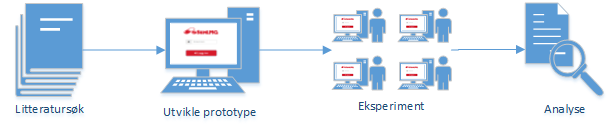
\includegraphics[width=10cm]{images/Arbeidsprosessen}
\caption{Arbeidsprosessen for masteroppgaven}
\label{fig:arbeidsprossen}
\end{center}
\end{figure}
\subsection{Fremdriftsplan}
For å finne rytmen og sikre fremdrift i prosjektet laget vi en fremdriftsplan. En fremdriftsplan skal vise når de forskjellige delene av prosjektet skal utføres og når de skal være ferdig. I vedlegg \ref{vedlegg:milep} ligger fremdriftsplanen. Denne er laget i form av en milepæleplan med et Gantt-skjema og illustrerer tidsplanen for prosjektet. 

Masteroppgave strekte seg på en tidsperiode fra 15.01.2016 til 01.06.2015. Underveis planla vi diverse oppgaver som måtte gjøres både før og etter selve utviklingen. Dette ville være oppgaver som å ha klart design og kravspesifikasjoner for prototypen, levere søknad til \gls{nsd} og analysere resultater av forsøk.
Alt som hadde med selve prototypen å gjøre valgte vi å markere med ekstra fet skrift i milepæleplanen. Dette var oppgaver som primært handlet om leveranser.  Vi valgte å lage et Gantt-skjema (Figur \ref{fig:ganttdiagram}) for å kunne få en bedre visualisering av tidsplanen. Her var det også rom for å bryte opp oppgaver fra milepæleplanen i mer spesifikke oppgaver med frister.
\begin{figure}[H]
\begin{center}
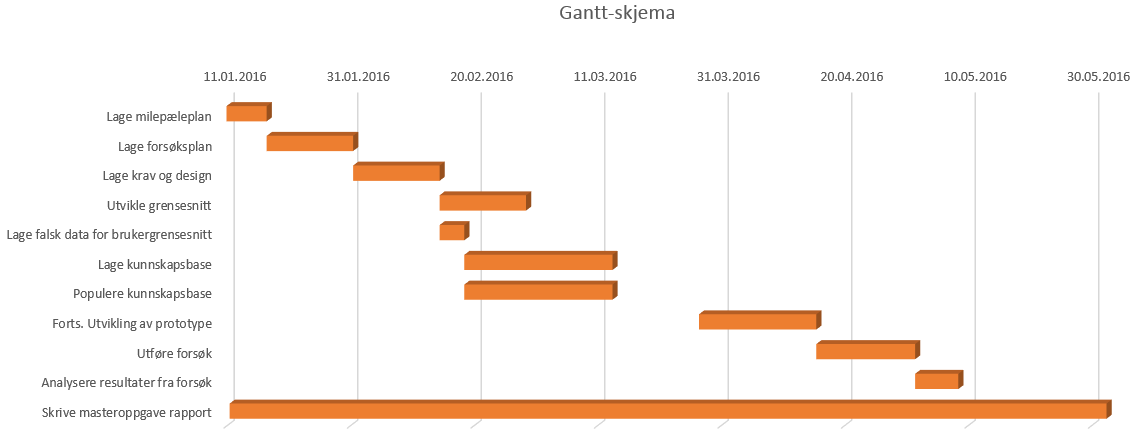
\includegraphics[width=16cm]{images/milep-gant-diagram}
\caption{Gantt-skjema over milepælene}
\label{fig:ganttdiagram}
\end{center}
\end{figure}
I et prosjekt som har en varighet på flere måneder er det essensielt å planlegge oppgaver underveis. Dette ville også være en god måte å unngå missforståelser. Med et Gantt-skjema vil alle være på samme bølgelengde, effektivt allokere og forstå relasjonene mellom oppgavene. Samtidig vil interessenter for prosjektet ha en felles forståelse for hva som er neste steg underveis i prosjektet.
\section{Arbeidsfordeling}

\section{Utvikling av prototypen}
 For å planlegge en prototype er det viktig å definere formålet med prototypen. Formålet med prototypen er å støtte legemiddelgjennomgang med forslag til tiltak for legemidler. For å kunne komme med forslag trengte prototypen å hente en kasuistikk, samstemme legemidler fra kasuistikken og dermed finne tiltak for legemidlene. Figur \ref{fig:formaalsbildeProto} er en konseptuell modell som beskriver hvert formål. Prototypen skulle bli brukt i et eksperiment og trengte derfor å bli utviklet etter dette formålet.
\begin{figure}[H]
\begin{center}

\includegraphics[width=14cm]{images/Formaalsbilde_prototype.png}
\caption{Konseptuell for prototypen}
\label{fig:formaalsbildeProto}
\end{center}
\end{figure}
\subsection{Kravspesifikasjoner}
Kravspesifikasjonen inneholder krav for å kunne bruke en slik prototype i et eksperiment. Et slik eksperiment ville kreve å ha målinger på hva deltakeren klikker på, hvilke tiltak som blir tatt og hvor lang tid deltakeren bruker.
\subsubsection{Brukergrensesnitt}
Da tyngden i prototypen ligger i tiltaksrepresentasjonen var det likevell viktig at prototypen var anvendbar, effektiv og tilfredstillende. Brukergrensesnittet skulle ha høy anvendbarhet slik at deltakere i stor grad kunne utføre de forhåndsbestemte oppgavene i eksperimentet. Den måtte også være effektiv slik at deltakere fort forstår hvordan det fungerer og klarer å navigere seg frem og tilbake på egenhånd. Det ønskes også at deltakere får en tilfredsstillende følelse ved å bruke prototypen.
\subsubsection{Tidsforbruk}
For å kunne bruke prototypen i et eksperiment måtte den måle tiden en deltaker bruker i prototypen under utførelsen av eksperimentet. Tidsforbruket som blir målet ville da kunne fungere som et tidsestimat på hvor lang tid en deltaker bruker på legemiddelgjennomgangen med prototypen.
\subsubsection{Lagring av skjema for legemiddelgjennomgang}
Når legemiddelgjennomgangen er ferdig skal det lagres i en database. Dette vil fungere som et resultat av legemiddelgjennomgangen og kan vurderes av en fagperson. 
\subsubsection{Lagring av klikk}
Lagring av klikk i grensesnittet kunne være et hjelpemiddel for analyse. Hva en person har klikket på kan i stor grad være til hjelp i å forstå hvordan en person har vurdert tiltakene. Prototypen skulle registrere at en deltaker har valgt å bruke tiltakene selv om personen har fjernet tiltaket i etterkant. Tiltakene har en kilde, og denne kilden skulle en deltaker kunne lese. Prototypen måtte derfor også registrere om en deltaker hadde klikket på kilden, noe som ville bety at deltakeren sannsynligvis hadde lest kilden.
\subsubsection{Spørreskjema}
Når deltakere er ferdig med å gjennomføre legemiddelgjennomgangen må systemet videresende deltakeren til et spørreskjema. Det var planlagt å ha et spørreskjema per kasuistikk. Prototypen må derfor kunne skille på kasuistikkene og videresende til riktig spørreskjema. Det måtte være en kobling mellom resultatet av legemiddelgjennomgangen og spørreskjema, derfor må det være et brukernavn for hver deltaker på hver kasuistikk. Dette brukernavnet må også vidersendes til og fylles ut automatisk i spørreskjema.

\subsection{Kasuistikker}
To kasuistikker skulle bli utarbeidet av våre biveiledere. Antallet ville være tilstrekkelig med tanke på at hver enkelt deltager skulle utføre to legemiddelgjennomganger. Kasuistikkene ga oss muligheten til å teste prototypen på ''reelle'' caser uten å bekymre oss om problemer rundt personopplysninger og pasientsikkerhet. Det var viktig at kasuistikkene inneholdte verdier på pasientspesifikk nyrefunksjon, enten i form av Estimert glomerulær filtrasjonshastighet (eGFR) eller utskillelse av kreatinin. Videre var det viktig at kasuistikkene som skulle bli utviklet var så virkelighetsnær som mulig, for å gjøre situasjonen ved bruken SemLMG så reell som mulig. 

\section{Utvikling av kunnskapsbase}
Prototypen krever en kunnskapsbase. Kunnskapsbasen vil ha strukturert informasjon som skal være tilgjengelig å bruke. Kunnskapsbasen vil være i form av en ontologi\ref{bakg:ontologi}

Det finnes ikke én korrekt metodikk for å utvikle en ontologi. I dette kapittelet ønsker vi å diskutere og vurdere en mulig prosess for å utvikle vår ontologi. Denne prosessen vil være en iterativ prosess som vil føre til et godt ontologidesign. Prosessen har vi adaptert fra en brukerveiledning som er skrevet ved Stanford University. \citep{ontology_101}
\subsection{Fastslå domenet og omfanget av ontologien}
Det første steget som må utføres er å definere domenet og omfanget for ontologien. For å gjøre dette vil vi stille oss noen basis spørsmål:
\begin{itemize}
\item Hva er domenet som ontologien skal dekke?
\item Hva er det ontologien skal brukes til?
\item Hvilke spørsmål er det ontologien skal svare på?
\item Hvem vil bruke og vedlikeholde ontologien?
\end{itemize}
Disse spørsmålene kan endre seg under ontologidesignet, men kan hjelpe oss til å avgrense omfanget til modellen vår. For å svare på disse spørsmålene er det naturlig å være i kontakt med interessenter og få en forståelse for hva systemet innebære og levere. Her har vi et godt utgangspunkt da vi har vært i mye kontakt med sektoren, veileder fra NTNU og våre bi-veiledere for masteroppgaven ved Sykehusapoteket i Midt-Norge. \\
En måte å definere omfanget på er å lage seg en liste over kompetansespørsmål. Dette er en liste som vil inneholde spørsmål som en kunnskapsbase skal kunne svare på. Dette er spørsmål som vil kunne fungere som en indikatortest for om ontologien inneholder nok informasjon slik at den kan svare på disse spørsmålene. Det er viktig å merke seg at disse spørsmålene er bare en slags kladd, og trenger ikke å være utfyllende. Før vi starter vår konstruksjon av ontologien vil vi definere disse kompetansespørsmålene for å ha et godt utgangspunkt.

\subsection{Bruk av eksisterende ontologier og informasjonskilder}
Det er nesten alltid lurt å vurdere å bruke eksisterende kilder og sjekke om vi kan raffinere og utvide disse til vårt formål. Dette kan være spesielt viktig om vårt system skal interagere med andre systemer eller vokabular. Det finnes allerede eksisterende ontologier og informasjonskilder som kan ha verdiskapning for oss. DrOn er en ontologi som vi kan ha nytte av å bruke. Om vi ikke bruker ontologien direkte så har DrOn modulære mønstre som vi kan adaptere inn i vår ontologi. Femstjerners FEST er også et interessant prosjekt og vi kommer til å ha kontakt med Statens Legemiddelverk både for tilgang til informasjonskilder og høre hvordan utviklingen går. ICD's internasjonale standard for felles terminologi og klassifisering av sykdommer er noe å betrakte. I vårt scenario ser vi på nyrefunksjonen. Ved å klassifisere sykdommen kan vi ved en senere anledning utvide kunnskapsbasen og rangere sykdommer. Et annen kilde for klassifikasjon er ATC. Dette kodeverket kan vi bruke for å gjøre effektive spørringer på hvilket organ legemidler påvirker samt virkemåte og egenskaper.

\subsection{Liste opp viktige begreper i ontologien}
Det kan være nyttig å liste opp viktige begreper som kan bli brukt i ontologien og i domenet. I vårt domenet ville det være naturlig å se på hva en medisin inneholder. Dette kan være begreper som virkestoff, dosering, interaksjon, indikasjon og bivirkning. Det kan også være nyttig å lage seg på begrepsapparatet innen farmasi. Når man skal liste opp slike begreper er det viktig å ikke tenke på overlapp eller hvilke relasjoner de har til hverandre. Det viktigste er å få listet de opp slik at de kan anvendes og moduleres senere.

\subsection{Definere klasser og klassehierarki}
Hvordan en tenker for å komme frem til klasser og klassehierarki er avhengig av et personlig synspunkt, og det er ingen metode som er bedre enn noen andre. Under vil vi liste opp tre mulige utviklingsprosesser for å oppnå et best mulig design av klasser:
\begin{itemize}
\item \textbf{Top-down} starter med det mest generelle konseptet i et domene, hvor du senere legger til videre spesialiseringer av konseptet. Man kan se for seg konseptet menneske. Hvor man kunne startet med å konstruere det mest generelle mennesket, og etterhvert spesialiserer hvilke kjønn eller raser som finnes.
\item \textbf{Bottom-up} starter med å definere de mest spesifikke klassene først, altså løvnodene i et typisk node-tre, og dermed grupperer disse spesifikke klassene i mer generelle klasser. Dette blir da motsatt tankegang av top-down.
\item En \textbf{kombinasjon} av disse to utviklingsprosessene er kanskje den mest vanligste måten å tenke på. Man starter med å definere det mest fremtredende først, dermed spesialiserer man superklasser og subklasser som tilhører denne. \\

\end{itemize}
Som sagt er dette personlig, og hvis en utvikler har et systematisk top-down syn på domenet, vil det være enklere å bruke top-down tilnærmingen. Kombinasjonprosessen er ofte enklere for mange ontologi utviklere. Dette kan være fordi konsepter som er fremtredende ofte er "midt-i", og disse er ofte mer deskriptive konseptene i et domene. \\

Det finnes ikke bare et eneste korrekt klassehierarkiet for et gitt domene. Hierarkiet avhenger av forskjellig bruk av ontologien, hvor detaljert den skal være for, personlige preferanser og noen ganger avhengigheter for å være kompatibelt med andre modeller. Det finnes flere retningslinjer for å sørge for at hierarkiet er mest mulig korrekt. Under konstruksjon av vår ontologi ønsker vi å ta hensyn til følgende retningslinjer: \\
\begin{itemize}
\item \textbf{Unngå klassesykluser:} En burde alltid unngå klassesykluser. En klassesyklus er typisk når du har en klasse A som har en subklasse B, og denne subklassen B er superklassen til klasse A. En slik situasjon tilsier at klasse A og klasse B er ekvivalent (alle instanser av A er instanser av B, og alle instanser av B er instanser av A). 
\item \textbf{Klasser og navn:} Det er viktig å skille på en klasse og navnet til en klasse. Navnet til en klasse kan endre seg hvis vi endrer terminologien, men begrepet er fortsatt et objekt i den virkelige verden. Et eksempel er hvis vi har et konsept som vi kaller \textit{Medisin}, men vi velger å endre navnet til \textit{Legemiddel} istedet. Klassen skal fortsatt representerer det samme konseptet, og alle tilhørligheter til konseptet skal bestå uten komplikasjoner.
\item \textbf{Entall/flertall versjoner av samme konsept:} En typisk feil å er å inkludere både entall og flertall versjoner av samme konsept. For eksempel ville det vært feil å definere en klasse \textit{Medisiner} og en subklasse \textit{Medisin}. Den beste måten å unngå slike feil er å forholde seg til enten entall eller flertalls navnekonvensjoner.
\end{itemize}
Disse er bare et fåtall av de retningslinjene som blir presentert i brukerveilederen som er utviklet på Stanford, men vi synes de omtalte retningslinjene er de mest sentrale for vårt prosjekt. \citep{ontology_101} Noen av de andre retningslinjene som blir presentert går på når en ny klasse bør bli introdusert og hvor mange subklasser er for mye eller for lite. Dette er vanlige problemstillinger når man holder på med datarelatert modellering, og veldig vanlig å ha i bakhodet under konstruksjon. Vi ønsker ikke å gå mer i detalj om dette i vår rapport.  

\subsection{Definere egenskaper til klasser}
Så langt har vi listet opp hvordan man går frem for å lage klasser og klassehierarkier. Klasser alene er ikke nok til å svare på kompetansespørsmålene som vi lister opp. For dette trengs det å defineres interne strukturer til objektene. Dette kalles egenskaper (properties), og vil hjelpe oss med å si noe mer om konseptene og relasjonene mellom dem.
Generelt sett finnes det flere typer objektegenskaper som kan bli egenskaper i en ontologi:
\begin{itemize}
\item Indre (intrinsic) egenskaper er verdier som er en naturlig del av et konsept. Dette kan for eksempel være øyenfargen på et menneske.
\item Utvendige (extrinsic) egenskaper er verdier som ikke er en naturlig del av et konsept. Dette er egenskaper som kommer fra "utsiden" av et konsept. Dette kan for eksempel være navnet på et menneske.
\item Hvis et konsept har en struktur er det naturlig å dele opp konseptet i deler. Dette er også egenskaper til et konsept, og disse delene kan være fysisk eller abstrakte elementer ved et konsept.
\item Forholdet til andre individer, dette er relasjoner mellom individer mellom medlemmer av klasser eller andre elementer.
\end{itemize}
Ettersom egenskaper arves på samme måte som objekt orientert arv, burde egenskaper tilhøre den mest generelle klassen i et klassehierarki. For eksempel burde øyenfarge være en del av klassen menneske, slik at subklassene mann og kvinne arver øyenfarge fra sin superklasse menneske. En mann og en kvinne arver øyenfarge fordi de begge er mennesker.

\subsection{Definere fasetter til egenskaper}
Egenskapene kan ha flere fasetter. Dette kan for eksempel være hvilke verdityper en egenskaper har eller hvor mange verdier som er lov (kardinalitet). Vi ønsker å liste opp noen fasetter som kan være viktige å tenke igjennom for å oppnå best mulig design: \\

\subsubsection{Kardinalitet}
Egenskapenes kardinalitet defineres som hvor mange verdier en egenskap kan ha. Noen systemer skiller mellom enkel (høyst en) og multippel (ethvert antall) kardinalitet. Et eksempel på dette kan være nesen og øyene til et menneske. Ved bruk av enkel kardinalitet for nesen vil et menneske kun ha en nese, mens ved bruk av multippel kardinalitet for øynene vil et menneske kunne ha to øyner. \\
Noen systemer tilater å a et maksimum og minimum kardinalitet på egenskaper. Dette er for å definere verdiene mer presist. Minimum kardinalitet av \textit{N} vil bety at en egenskap må ha minst \textit{N} verdier, mens maksimum kardinalitet på \textit{M} vil bety at en egenskap kan ha maks \textit{M} verdier. \\

\subsubsection{Relasjonsmønstre til en egenskap}
Ved konstruksjon av egenskaper må det vurderes om egenskapens relasjoner skal ha restriksjoner som sier noe om relasjonsmønsterert til egenskapen. Disse restriksjonene blir uttrykt ved å bruke domain og range attributtene. Restriksjonene vil si noe om hvilke klasser en egenskap tilhører. Et utsagn om at to individer har en relasjon til hverandre via en spesiell egenskap kan bære med seg ekstra implisitt informasjon om disse individene og konklusjoner kan trekkes.


